%!TEX root = masters-dissertation.tex
\chapter{StarCraft}
\label{chapter:sc}

\emph{Real-time strategy} (RTS) are computer games in which multiple players control teams of characters and resources over complex simulated worlds where their actions occur simultaneously (so there is no turn-taking between players). 
Players often compete over limited resources in order to strengthen their team and win the match. 
As such, RTS games are an interesting field for AI, because the state space is huge, actions are concurrent, and part of the game state is hidden from each player. 
Game-play involves both the ability to manage each unit individually \textit{micro-management}, and a high-level strategy for building construction and resource gathering (\textit{macro-management}). 

\textit{StarCraft} is an RTS created by \textit{Blizzard Entertainment, Inc.}\footnote{
StarCraft website in Blizzard Entertainment, Inc. \url{http://us.blizzard.com/pt-br/games/sc/}}.
In this game, a player chooses between three different races to play (illustrated in Figure~\ref{fig:sc-races}), each of which having different units, buildings and capabilities, and uses these resources to battle other players, as shown in Figure~\ref{fig:sc-fight}. 
% 
\begin{figure}[ht]
\centering
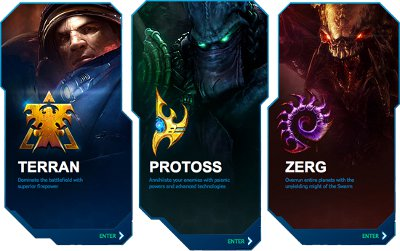
\includegraphics[width=400px]{images/sc-races}
\caption{StarCraft: Brood War --- Race selection screen.}
\label{fig:sc-races}
\end{figure}
% 
The game consists on managing resources and building an army of different units to compete against the armies built by opposing players. 
Units in the game are created from structures, and there are prerequisites for building other units and structures. 
Consequently, one key aspect of the game is the order in which buildings and units are built, and good players have strategies to build them so that specific units are available at specific times for attack and defense moves. 
Such building strategies are called \textit{build orders} or \textit{BOs}. 
Strong BOs can put a player in a good position for the rest of the match.
BOs usually need to be improvised from the first contact with the enemy units, since the actions become more dependent on knowledge obtained about the units and buildings available to the opponent~\cite{hagelback2012potential,churchill2011build}. 
% 
\begin{figure}[ht]
\centering
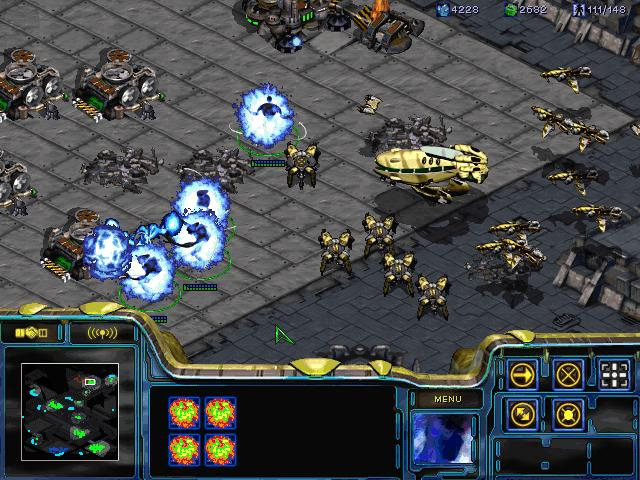
\includegraphics[width=400px]{images/sc-fight}
\caption{StarCraft: Brood War --- Batttle Scene.}
\label{fig:sc-fight}
\end{figure}